\documentclass{article}
\usepackage[utf8]{inputenc}
\usepackage[document]{ragged2e}
\usepackage{hyperref}
\usepackage{tikz}
\usepackage{pifont}
\graphicspath{{/home/feideu/Work/Gnunet/schemafuzz/docs/}}
\usepackage{graphicx}
\usepackage{emp}
\usetikzlibrary{shapes.arrows,chains}
\usepackage[ngerman]{babel}

\title{Documentation for schemaFuzz}
\author{Ulrich "Feideus" Erwan}

\begin{document}
\begin{empfile}
	
\maketitle Documentation For SchemaFuzz
	\section{Summary?}
		This document actually needs a front page.
	\section{Introduction}
	
SchemaFuzz is a free software command line tool incorporated inside the Gnu Taler package 
which is a free software electronic payment system providing anonymity for customers.
The main goal of this project is to provide an effecient debbuging tool that uses a "fuzzing" strategy oriented on databases.  
Traditionnal fuzzing is defined as "testing an automated software testing technique that involves providing invalid, unexpected, or random data as inputs to a computer program". SchemaFuzz uses this principle and applies it to the database field.
Where a traditionnal fuzzer would send malformed input to a program, SchemaFuzz modifies the content of a database to test that program's behavior when stumbling on such unexpected data. \\*
Obviously, this tool is meant to be used as a mean of debugging as the goal is to pop buggs or put into light the security breaches that the code may contain regarding the retrieving, usage and saving of a database's content.
As this tool is being developped as a master's thesis project, its current state is far from being finished and there are many options and optimisations that deserve to be implemented that are not yet available.
These future/missing features will be detailed and discussed in a dedicated section.

	
	\section{Context and Perimeter}
SchemaFuzz's developpement enrolls in the global dynamic of the past decades regarding internet  that sustain great efforts to make it a more fluid, pleasant but more importantly a safer space. This tool is meant to help developpers, mainteners and more genericly anyone that makes use of database comming from a database under his influence in their task. A good way to summerise the effect of this tool is to compare it with an "cyber attack simulator".
This means that the idea behind it is to emulate the damage that an attacker may cause subtly or not to a database he unlegitly gained privileges on. This might in theory go from a simple boolean flip (subtle modifications) to removing/adding content to purely and simply destroying or erasing all the content of the database.
SchemaFuzz focuses on the first part : modification of the content of the database by single small modification that may or may not overlap. These modifications may be very aggressive of very subtle.
It is intresting to point out that this last point also qualifies SchemaFuzz as a good "database structural flaw detector".
That is to say that errors typically triggered by a poor management of a database (wrong data type usage, incoherence beetween database structure and use of the content etc ...) might also appear clearly during the execution.   
		\subsection{Perimeter}
		\begin{figure} [htbp]
		\centering
		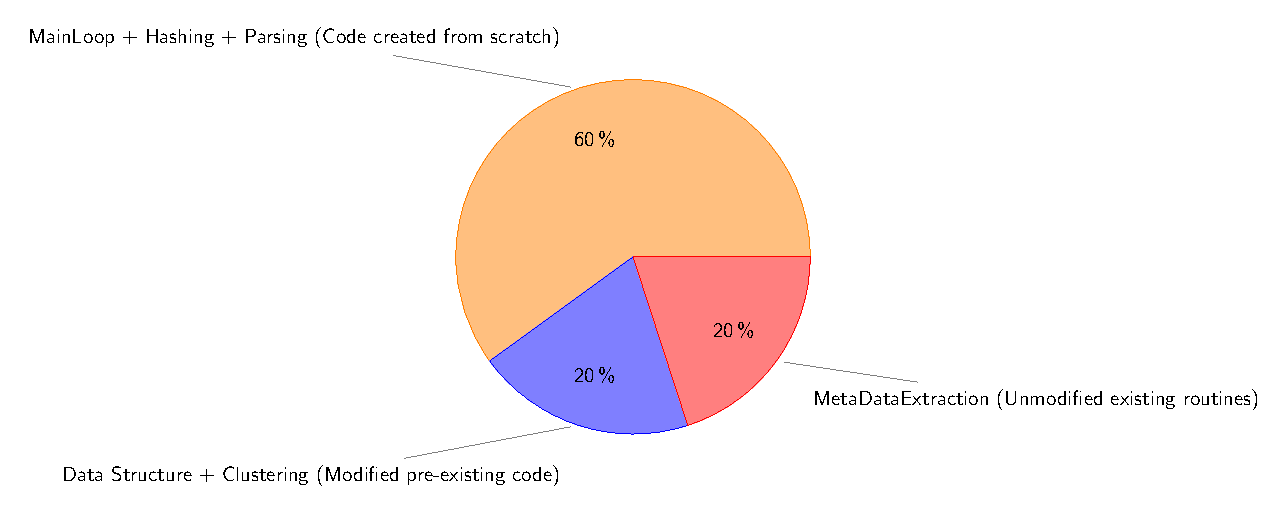
\includegraphics[scale=1]{codeOriginDiagram.pdf}
		\caption{Shows the nature of the code for every distinct component. The slice size is a rough estimation.}
		\end{figure}
		\subsection{When to use it}
SchemaFuzz is a very usefull tool for anyone trying secure a piece of software that uses database ressources. The target software should be GDB compatible and the DBMS has to grant access to the target database through credentials passed as argument to this tool.

---It is very strongly advice to use a copy of the target databas erather than on the production material. Doing so will very likely result in the database being corrupted and not usable for any usefull mean.--
 
	\section{Usage}
		\subsection{prerequisites}
			SchemaFuzz requires the presence of a list of libraries to work properly which are :
			\begin{itemize}
			\item org.apache.commons.math3 >= 3.6
			available at \\*
			\url{https://commons.apache.org/proper/commons-math/download_math.cgi}			
			\end{itemize}
The library has to be installed in the maven repository to be available. The instructions detailed at the following address explain how to do that. futher information can be found on the official maven website.\\*

			\url{https://www.mkyong.com/maven/how-to-include-library-manully-into-maven-local-repository/}
			
		\subsection{setting up the code}
			Once all the depencies have been installed successfully, clone the source available on the official git taler repository \\*
			\url{https://git.taler.net/schemafuzz.git}
			\begin{verbatim}
			 git clone https://git.taler.net/schemafuzz.git
			\end{verbatim}
			
the folder containing the code shoud hold the rights for reading writing and executing (rwx) for the user that plans to run the tool.
if this is not the case, you can give these rights like so
			\begin{verbatim}
			sudo chmod -R 700 schemafuzz
			\end{verbatim}
		\subsection{Building}
SchemaFuzz is using maven for building and library management purposes.
Therefore, using the maven command line building script is way to go.
Standard way of building :\\*
			\begin{verbatim}
			./mvnw package
			\end{verbatim}
				
This maven building method also offers alternative instructions for 	more precise/refined way of building as well as compilation and test 
launching options (those should only be intresting for the contributors).

Launching the test suit :\\*
			\begin{verbatim}
			./mvnw test
			\end{verbatim}
Compiling the code :\\*		
			\begin{verbatim}
			./mvnw compile
			\end{verbatim}
		
Other usefull commands: \\*		
		
			\begin{verbatim}
			./mvnw clean
			\end{verbatim}
			\begin{verbatim}
			./mvnw validate
			\end{verbatim}
			\begin{verbatim}
			./mvnw deploy
			\end{verbatim}
		
		\subsection{Setting up the database}	
	
Launch the "dbConfigure" script.
			\begin{verbatim}
				./dbConfigure
			\end{verbatim}		 
	
	\section{Design}
		\subsection{Generic explanation}
SchemaFuzz implementation is based on some bits of the SchemaSpy project source code.
The majority of this project is built on top of this already existing code and is organised as follows :
		\begin{itemize}
		\item{mutation/data-set used as a way to store the imputs,outputs and other intresting data from the modification that was performed on the target database}
		\item{the mutation Tree, used to store the mutations coherently}
		\item{an analyser that scores the mutations to influence the paths that will be explored afterwards}
		\end{itemize}
		 
This organisation will be detailled and discussed in the following sections.
		\subsection{SchemaSpy legacy/metadata extraction}
SchemaSpy source code has provided the metadata extraction routine. The only job of this routine is to initialise the connection to the database and retrieve its metadata at the very beginning of the execution (before any actual SchemaFuzz code is run). These metadata include data types, table and table column names, views and foreign/primary key constraints. Having this pool of metadata under the shape of java objects allows the main program to properly frame what the possibilities are in terms of modifications as well as dealing with the possible constraints on the different tables. The modifications that will be created during the main loop will be designed to respect the frame built for the result of this extraction.

Exemple of typical metadata Set 


\begin{figure} [htbp]
\centering
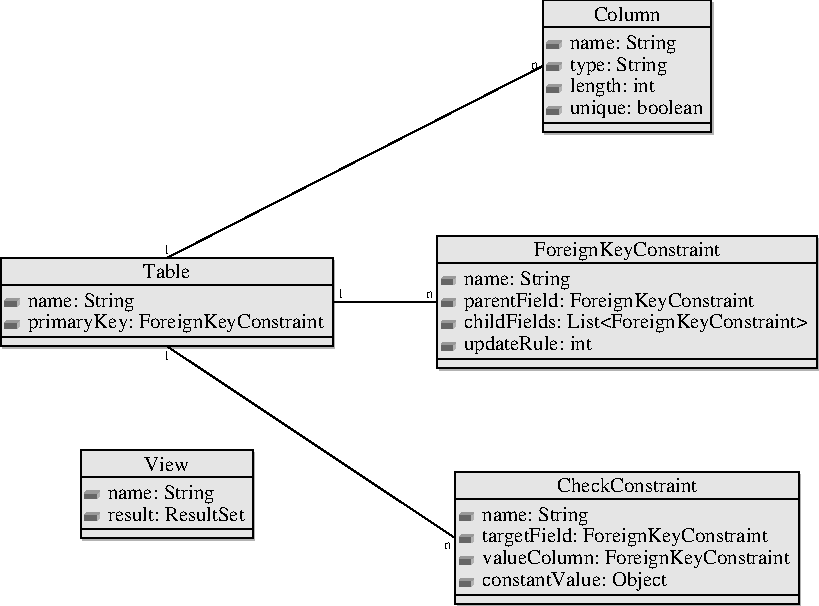
\includegraphics[scale=1]{MetaDataExtractionDiagram-1.pdf}
\caption{Objects returned by the metadata extraction routine.}
\end{figure}

In order to do that, the user shall provide this set of mandatory database related arguments
			\begin{itemize}
 				\item The driver to the corresponding database RDBMS (only support PostGres at the moment)
 				\item The credentials to be used to access the database.
 				\item The name of the database (duh)
			\end{itemize}
		\subsection{SchemaFuzz Core}		
			\subsubsection{Constrains}
The target database often contains contraints on one or several tables. These constraints have to be taken into account in the process of fabricating mutations as most of the time they restrict the possible values that the pointed field can take. This restriction can take the shape of a \underline {Not Null} constraint, \underline{Check} constraint, {Foreign key} constraint (value has to exist in some other table's field) or \underline{Primary key} constraint (no doublets of value allowed). These constraints are stored as Java objects instanciated from the corresponding class.

\begin{figure} 
\centering
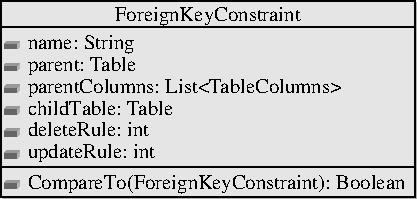
\includegraphics[scale=1]{ForeignKeyClassDiagram-1.pdf}
\caption{Objects returned by the metadata extraction routine.}
\end{figure}

The last two ones are the problematic ones. They imply specific work before applying any mutations to make sure that the value respect all the restrictions. before doing anything else after the metadata extraction is done, SchemaFuzz performs an update of all the existing constraints on the database to add the CASCADE clause. This allows the values bonded by a foreign key constraints to take effect. This update reverts to take the constraints back to their initial state before the program exits.
				\paragraph{Primary key contraints (PKC)} :
The primary key constraints require an extra DB query that checks the existence of the value in the column. If the value already exists (the query's result is not empty), the mutation will be dropped before being executed.
				\paragraph{Foreign key contraints (FKC)} :
The foreignKey constraint is the trickiest one. Its inherent nature bonds two values of different table column where the value being referenced is called the father, and the referecing field, the child. To be precise, in order to change one of the two values, the other has to be changed accordingly in the same statement.SchemaFuzz uses the power of the CASCADE clause to make the change possible. This clause allows the DRBMS to automaticly change the value of the child if the father has been changed.
This mechanic allows to change any of the bounded values by changing the father's value.
To do so, the software has a way to tranfert the mutation from a child to its parent (called the mutationTransfert).

  				
			\subsubsection{Mutations}
				\paragraph{What is a Mutation}
A mutation is a Java object that bundles all the informations that are used to perform a modification in the database. Every is linked to its parent and inherits some of his parent's data. In the case of a follow up mutation the child inherits the the database row that was his parent's target.Therefore the initial state (state before the injection of the modification) of its target is exactly the final state (state after injection of the modification) of his parent's target. A mutation is created for each iteration of the main loop and represents a single step in the progress of the fuzzing.
It also holds the informations concerning the result of the injection in the shape of a data vector. This data vector is then used to perform a clustering calculus to determine the "uniqueness" of the mutation. This value is also stored inside the mutation object and is used as the weight of this mutation in the tree.

\begin{figure} 
\centering
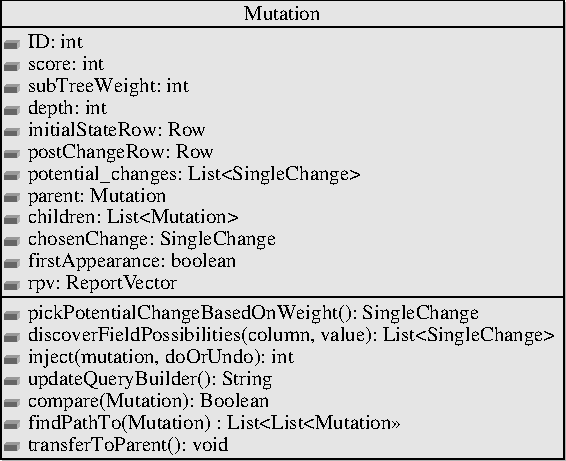
\includegraphics[scale=1]{MutationClassDiagram-1.pdf}
\caption{Structure of a Mutation}
\end{figure}

  				
				\paragraph{Choosing patern}
For each iteration of the main loop, a modification has to be picked up as the next step in the fuzzing proccess. This is done by concidering the current state of the tree.
Three parallel code paths can be triggered from this point.
				\begin{itemize}
				\item{Continue on the current branch of the tree (triggered if the last mutation scored better than its parent)}
				\item{Pick an existing branch in the tree and grow it (triggered if the last mutation scored worse than its parent on a 50/50 chance with the next bullet)}
				\item{Start a new branch (triggered if the last mutation scored worse than its parent on a 50/50 chance with the previous bullet)}
				
\begin{figure} 
\centering
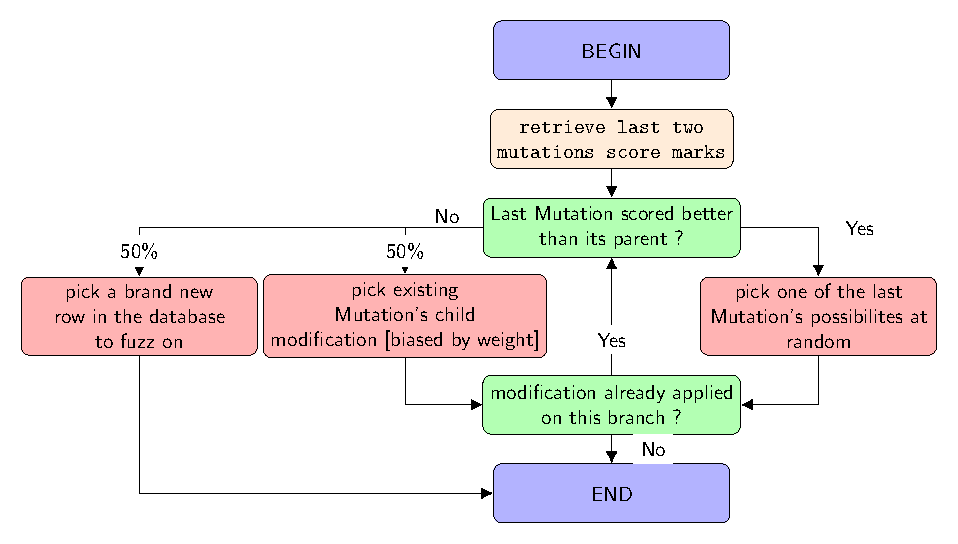
\includegraphics[scale=1]{pickingPaternDiagram.pdf}
\caption{picking Patern schema}
\end{figure}				
				
				\end{itemize}
A branch is a succession of mutation that share the same database row as their modification target.
The heuristics determining the next mutation's modification are still very primitive and will be thinly ajusted in futures versions.								 
				\paragraph{Creating malformed data} 
As the goal of running this tool is to submit unexpected or invalid data to the target software it is necessary to understand what t
Fuzzing a complex type such a timestamp variable has nothing to do with fuzzing a trivial boolean. In practice, A significant part o
and this matter could absolutly be the subject of a more abstract work. We focused here on a very simple approach (as a first step).
After retrieving the current row being fuzzed (may it be a new row or a previously fuzzed row), the algorithm explores the different
The algorithm then builds the possible modification for each of the fields for the current row.
At the moment, the supported types are : % add a list of the supported types.
More primitives types will be added in the future.
The possible modifications that this tool can produce at the moment are : % add complete list of the modifications that CAN be gener$
				Int Types:
				\begin{itemize}
		
					\item Extreme values (0-32676 (int) etc...)
					\item Random value (0<value<32676 (int) etc...)
					\item Increment/Decrement the existing value (332 -> 333 OR 332 -> 331)
				\end{itemize}
				String Types:
				\begin{itemize}
			
					\item Change string to "aaa" ("Mount Everest" -> "aaa")
					\item Increment/Decrement ASCII character at a random position in the string ("Mount Everest" -> "Mount Fverest")
					Boolean
					\item Swaping the existing value (F -> T OR T -> F)
					\end{itemize}
					Date Types : (! IMPLEMENTED BUT NOT FULLY FUNCTIONNAL)					
					\begin{itemize}
					\item Increment/Decrement date by 1 day/minutes depending on the precision of the date
					\item Set date to 00/00/0000
				\end{itemize}
Obviously, these "abnormal" values might in fact be totally legit in some cases. in that case the analyzer 
will rank the mutation rather poorly, which will lead to this tree path not being very likely to be developped further more.
				\\*
				\paragraph{Sql handling}
All the SQL statements are generated within the code. This means that the data concerning the current and future state of the mutations have to be very precise. Otherwise, the SQL statement is very likely to fail. Sadly, since SchemaFuzz only supports postgreSQL, the implemented synthax follow the one of postgres
DBMS. This is already a very big axis for future improvements and will be detailled in the dedicated section.
The statement is built to target the row as precisely as possible, meaning that it uses all of the non fuzzed values from the row to avoid updating other row accidently. Only the types that can possibly be fuzzed will be used in the building of the SQL statement. Since this part of the code is very delicate in the sense that it highly depends on an arbitrary large pool of variables from various types it is a good bugg provider. 
				
				\paragraph{Injecting} :
The injection process sends the built statement to the DBMS so that the modification can be operated. After the execution of the query, depending of the output of the injection (one modification, several modifications, tranfer) informations are updated so that they can match the database state after the modification. If the modification failed, no trace of this mutation is kept, it is erased and running goes on like nothing happenned.  				
				\paragraph{Special Case(MutationTransfert)} :
The mutation tranfert is a special case of a modification being applied to the database.
It is triggered when the value that was supposed to be fuzzed is under the influence of a FKC as the child.
In the case a FKC (In CASCADE mode), only the father can be changed, which also triggers the same modification on all of his children. The algorithm then "transfers" the modification from the original mutation to its father.
After injecting the transfered mutation, the children mutation is indeed modified but the modification "splashed" on some parts of the database that was not meant to be changed.
Hopefully, this does not impact the life of the algorithm until this mutation is reverted (see next paragraph).
				\paragraph{Do/Undo routine} :
The Do/Undo mechanism is at the center of this software. Its behavior is crucial for the execution and will have a strong impact on the coherence of the data nested in the code or inside the target database throughout the runtime.
This mechanism allows the algorithm to revert a previous mutation or, if necessary inject it one more time. 
Undoing a mutation applies the exact opposite modification that was originally applied to the database ending up in recovering the same database state as before the mutation was injected.
Reverting mutations is the key to flawlessly shifting the current position in the mutation tree.
The case of the transfered mutation is no exception to this. In this case, the mutation applied changes on an unknown number of fields in the database. But, the FKC still bounds all the children to their father at this point (this is always the case unless this software is not used as intended).  
Changing the father's field value back to its original state will splash the original values back on all the children.
This mechanism might trigger failing mutations in some cases (usually mutations following a tranfer). This issue will be addressed in the known issues section. 
			\subsubsection{Tree Based data structure}
All the mutations that are injected at least once in the course of the execution of this software will be stored properly in a tree data structure. Having such a data structure makes parent-children relations between mutations possible. The tree follows the traditionnal definition of the a n-ary algorithmic tree.
It is made of nodes (mutations) including a root (first mutation to be processed on a field selected randomly in the database)  
Each node has a number of children that depends on the ranking its mutation and the number of potential modifications that it can perform.
				\paragraph{Weight} :
Weighting the nodes is an important part of the runtime. Each mutation has a weight that is equal to the analyzer's output. This value reflects the mutation's value. If it had an intresting impact on the target program behavior (if it triggered new buggs or uncommon code paths) than this value is high and vice-versa. The weight is then used as a mean of determining the upcomming modification. The chance that a mutation gets a child is directly proportionnal to its weight.
This value currently isn't biased by any other parameter, but this might change in the future.  
				\paragraph{Path}
Since the weighting of the mutation allows to go back to previously more intresting mutations, 
there is a need for a path finder mechanism. Concretly, this routines resolves the nodes that separate nodes A and B in the tree. A and B might be children and parent but can also belong to complitely different branches. This path is then given to the do/undo routine that processes back the modifications to set the database up in the required state for the upcomming mutation. 

\begin{figure} 
\centering
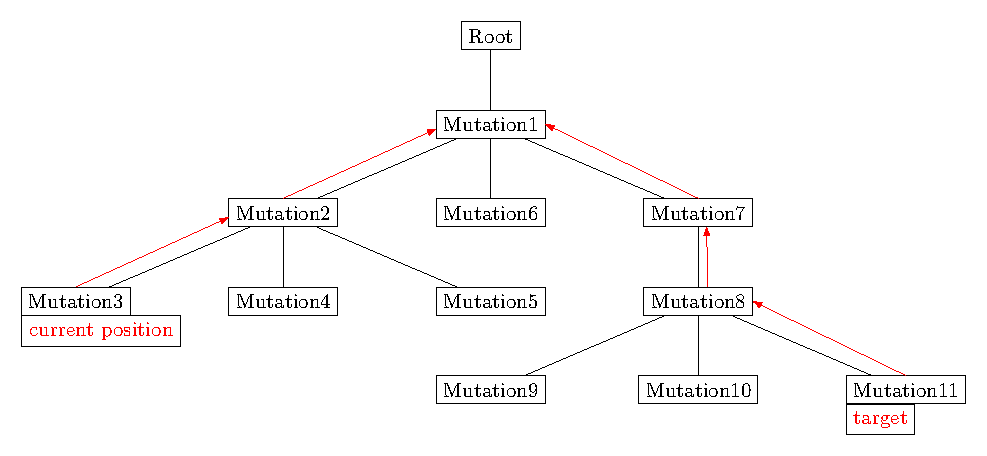
\includegraphics[scale=1]{CommonAncestorDiagram.pdf}
\caption{Objects returned by the metadata extraction routine.}
\end{figure}
			\subsubsection{The analyzer}
Analyzing the output of the target programm is another critical part of SchemaFuzz. The analyzer parses in the stack trace of the target software's execution to try measuring its interest. The main criteria that defines a mutation intrest is its proximity to previously parsed stack traces. The more distance between the new mutation and the old ones, the better the ranking. 
				\paragraph{Stack Trace Parser}
The stack trace parser is a separate Bash script that processes stack traces generated by the GDB C language debugger and stores all the relevent informations (function's name, line number, file name) into a Java object. The parser also generates as a secondary job a human readable file for each mutation that synthetises the stack trace values as well as additionnal intresting information usefull for other mechanisms (that also require parsing). These additionnal informations include the path from root to mutation (usefull for rolling back the database to a specific state).
				\paragraph{Hashing}
In order to be used in the clustering algorithm, the stack trace of a mutation has to be hashed.
Hashing is usually defined as follows : 
				\begin{quotation}
"A hash value (or simply hash), also called a message digest, is a number generated from a string of text. The hash is substantially smaller than the text itself, and is generated by a formula in such a way that it is extremely unlikely that some other text will produce the same hash value."
				\end{quotation}
				
In the present case, we used a different approach. Since proximity beetween two stack traces is the key to a relevant ranking, it is mandatory to have a hashing function that preserves the proximity of the two strings. 
In that regards, we implemented a version of the Levenshtein Distance algorithm.
This algorithm can roughly be explain by the following :
				\begin{quotation}
"The Levenshtein distance between two words is the minimum number of single-character edits (insertions, deletions or substitutions) required to change one word into the other."
				\end{quotation}				 
After hashing the file name and the function name into numerical values trough Levenshtein distance, we are creating a triplet the fully (but not fully accuratly yet) represents the stack trace that is being parsed. This triplet will be used in the clustering method. 

\begin{figure} 
\centering
\begin{tabular}{ | l | l | l | l | l | l | c | r | }
  \hline			
  E & X & E & M & P & L & E &  \\ \hline
  \ding{51}  & \ding{51}  & \ding{56}  & \ding{51}  & \ding{51}  & \ding{51}  & \ding{51} & \ding{56}  \\\hline
  E & X & A & M & P & L & E & S \\
  \hline  
\end{tabular}
\caption{Exemple of the levenshtein distance concept.}
\end{figure}

The Distance for this exemple is 2/8x100

				\paragraph{The Scoring mechanism}
The "score" (or rank) of a mutation is a numerical value that reflects its intrest. This value is calculated through a modified version of a clustering method that computes an n-uplet 			into a integer depending on the sum of the euclidian distances from the n-uplet to the existing centroids (groups of mutation's n-uplets that were already processed).
This value is then set as the mutation's rank and used as a mean of chosing the upcomming mutation.
\begin{figure} 
  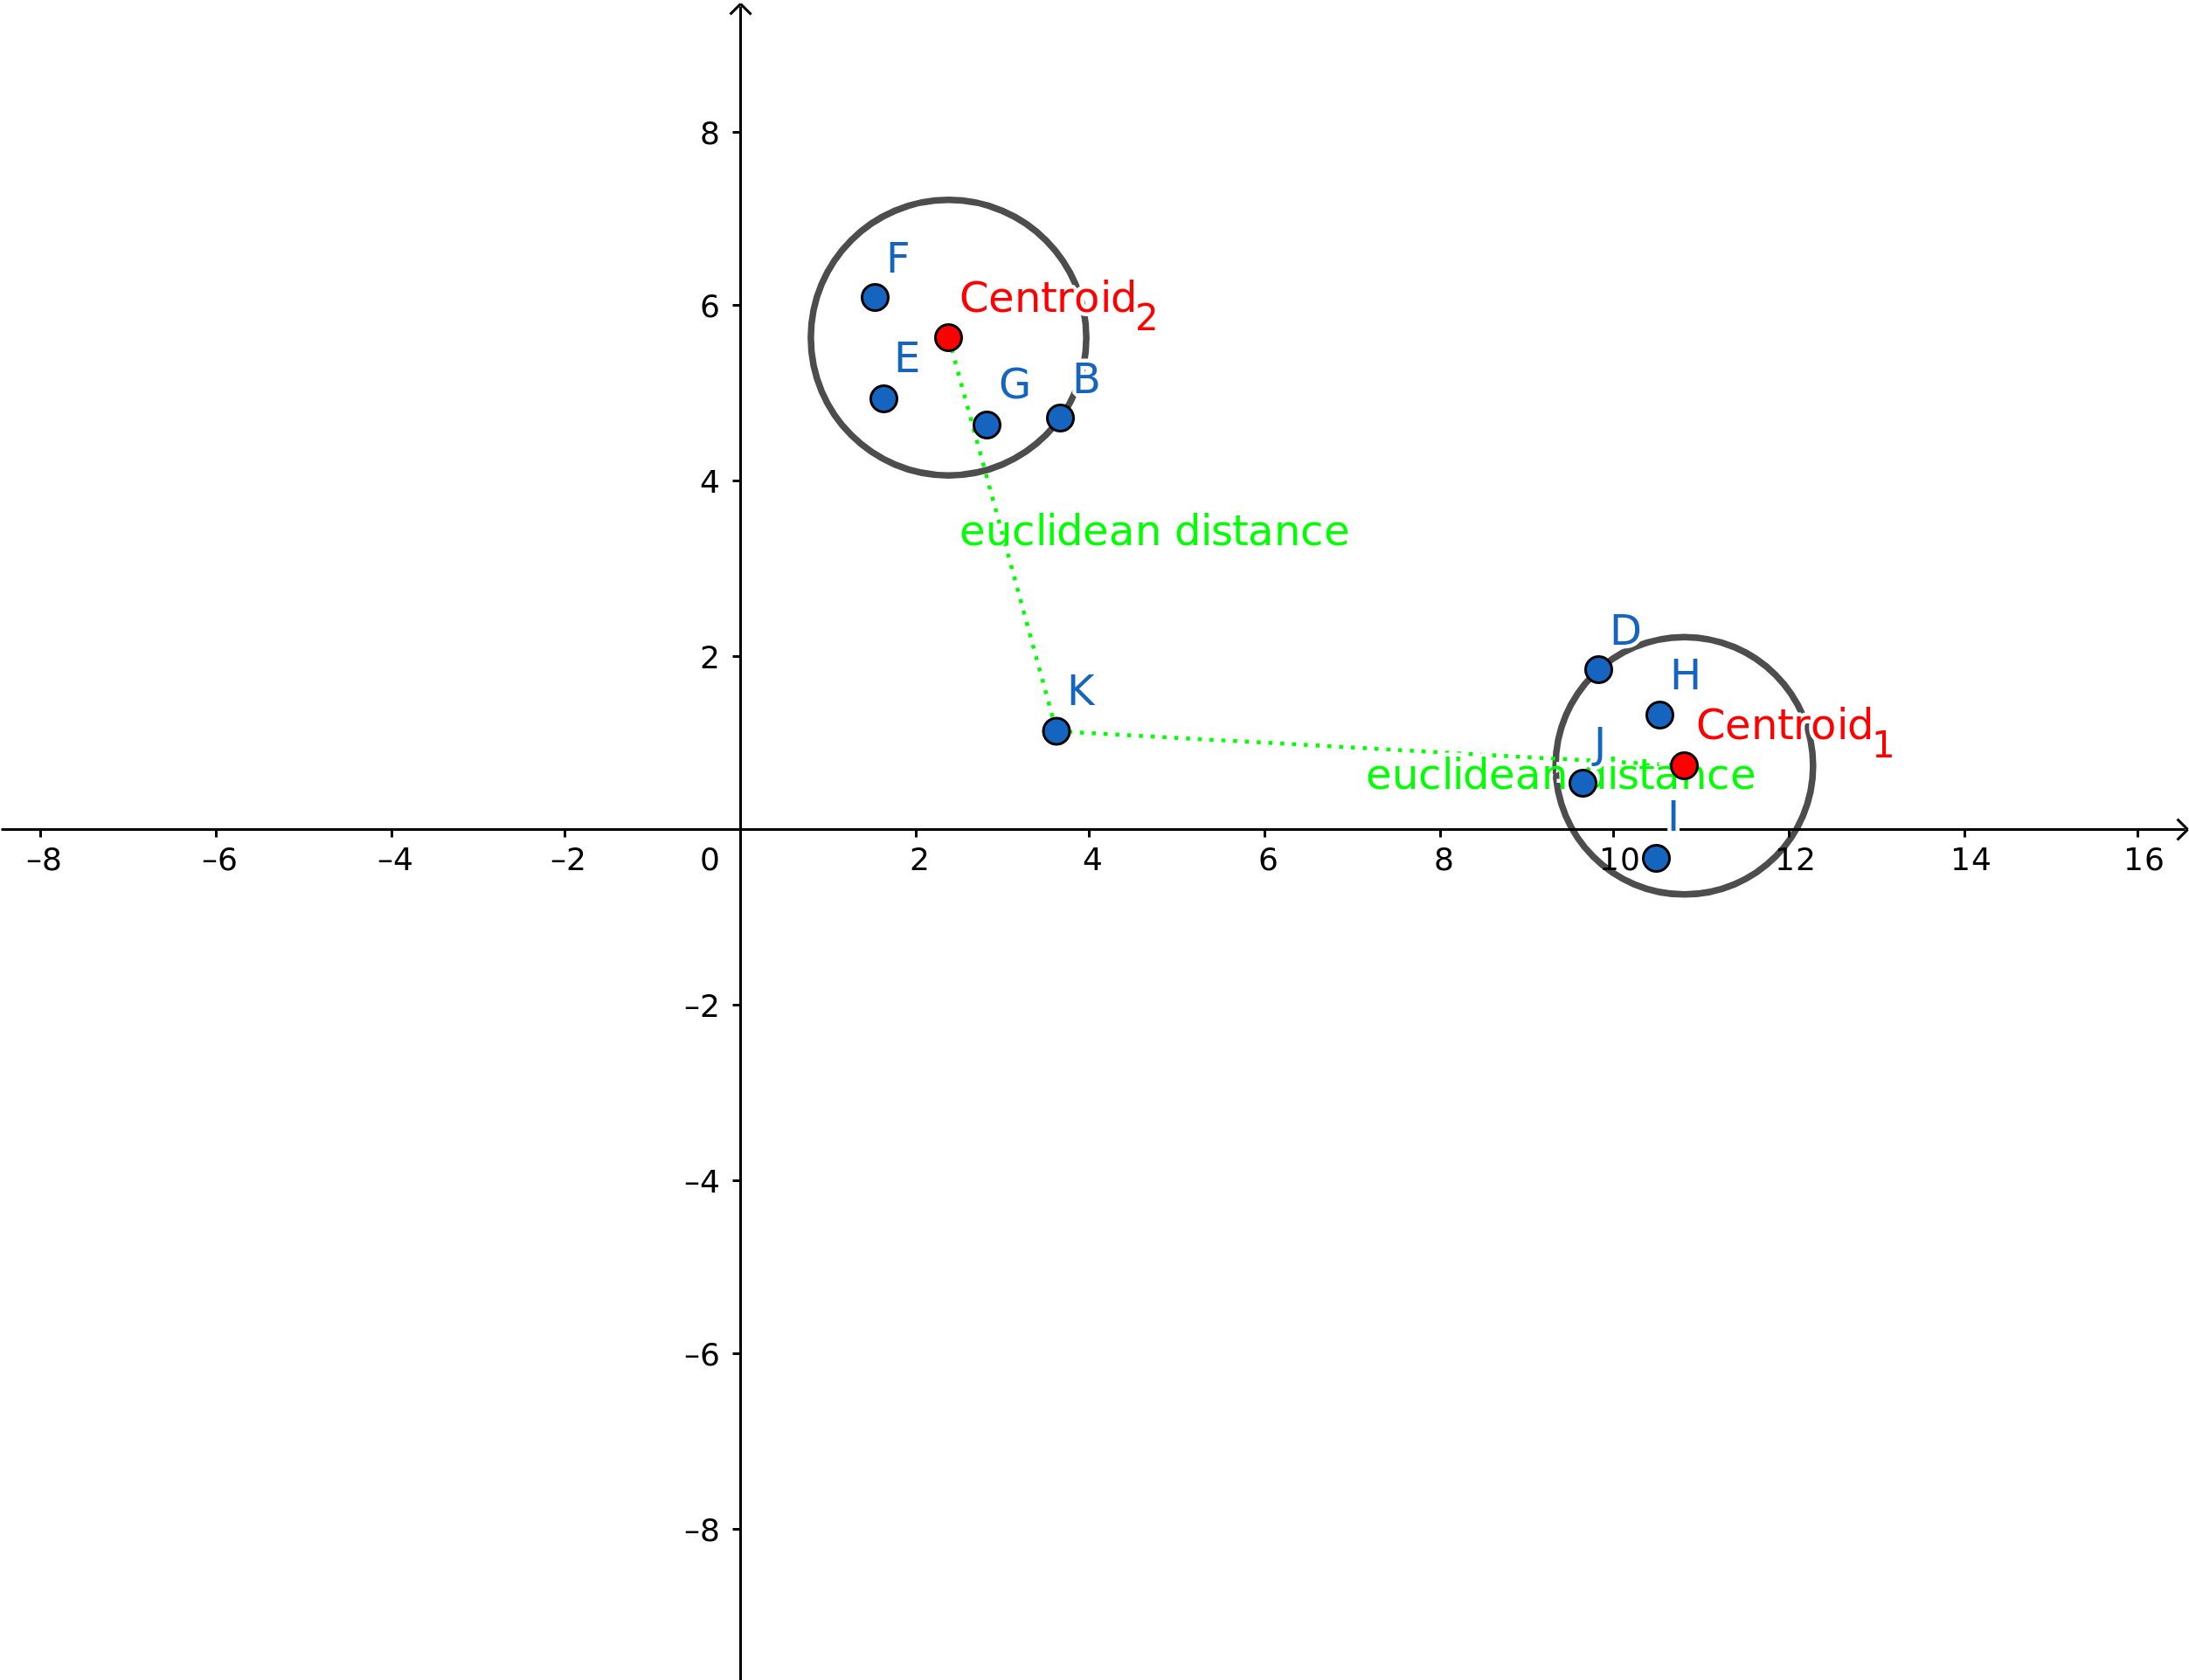
\includegraphics[width=\textwidth]{Scoring.png}
\end{figure}	
		\subsection{Known issues}		
About one mutation out of 15 will fail for unvalid reaseons.
			\subsubsection{Context Cohorence}
A significant amount of the failing mutations do so because of the transfer mechanism. As said in the dedicated section, this mechanism applies more than one change to the database (Potentially the whole database). In specific case, this property can become problematic. 
More specificaly, when the main loop identifies a mutation's child as the upcomming mutation and its parent row has been splashed with the effect of a transfer. In this case, the data embedded in the schemaFuzz data structure may not match the data that are actually in the database, this delta will likely induce a wrongly designed SQL statement that will result in a SQL failure (meaning that 0 row were updated by the statement).
			\subsubsection{Foreign Key constraints}			
For a reason that is not yet clear, some of the implied FKC of the target database can't be properly set to CASCADE mode. This result in a FKC error (mutation fails but the program can carry on)			
			\subsubsection{Tests}
Besides the test suit written by the SchemaSpy team for their own tool (still implemented in SchemaFuzz for the meta data extraction), the tests for this project are very poor. Their are only very few of them and their utility is debatable. This is due to the lack of experience in that regard of the main developper. Obviously, we are very well aware of this being a really severe flaw in this project and will be one of the main future improvements.
This big lack of good maintenance equipment might also explain some of the silent and non silent buggs that still remain in the code to this day.

			\subsubsection{Code Quality}
We are well aware that this tool's source code is of debatable quality. This fact induces the  buggs and unexpected behaviors discussed earlier on some components of this program. 
The following points constitute the main flaw of the source code:
			\begin{itemize}
			\item Hard to maintain. The code is not optimised either in term of size or 			efficency. Bad coding habits tend to make it rather weak and unstable to context changes.
			\item Structure is not intuitive. The main loop of the program lacks a good 		structure.
			\end{itemize}
 			
	\section{Upcomming features and changes}
This section will provide more insights on the future features that might/may/will be implemented as well as the changes in the existing code.
Any sugestion will be greatly appriciated as long as it is relevent and well argumented. All the relevent information regarding the contributions are detailled in the so called section.
	
		\subsection{Code coverage}
We are considering changing or simply adding code coverage in the clustering method as a parameters.Not only would this increase the accuracy of the scoring but also increase the accuracy of the "type" of each mutation. To this day, this tool does not make a concrete difference in terms of scoring or information generating (reports) beetween a mutation with a new stack trace in a very common code path and a very common stack trace in a very rarely triggered code path.
		\subsection{Centralised anonymous user data}
SchemaFuzz's efficiency in thightly linked to the quality of its heuristics. this term includes the following points 
		\begin{itemize}
		\item{Quality of the possible modifications for a single field}
		\item{Quality of the possible modifications for each data type}
		\item{Quantity of possible modifications for a single field}
		\item{Quantity of supported data types}
		\end{itemize}
Knowing this, we are also concidering for futures enhancements an anonymous data collection  for each execution of this tool that will be statisticly computed to determine the best modification in average. This would improve the choosing mechanism by balancing the weights  depending on the modifcation's average quality. Modifications with higher average quality would see their weight increased (meaning they would get picked more frequently) and vice versa. 			
	\section{Contributing}
You can send your ideas at  \\*
		\url{erwan.ulrich@gmail.com}
Or directly create a pull request on the official repository to edit this document and/or the code itself
	\section{Conclusion}
\end{empfile}
\end{document} 
